\section{Test Description and Success Criteria}
The tests are located in \texttt{simulation/dynamics/reactionWheels/\_UnitTest/\newline
test\_reactionWheelStateEffector\_integrated.py} \textbf{and} \texttt{simulation/dynamics/reactionWheels/\newline\_UnitTest/
test\_reactionWheelStateEffector\_ConfigureRWRequests.py}. Depending on the test, there are different success criteria. These are outlined in the following subsections:
\subsection{Balanced Wheels Scenario - Integrated Test}
In this test the simulation is placed into orbit around Earth with point gravity, has 3 reaction wheels attached to the spacecraft, and the wheels are in ``Balanced" mode. Each wheel is given a commanded torque for half the simulation and the rest of the simulation the torques are set to zero. The following parameters are being tested:
\begin{itemize}
	\item Conservation of orbital angular momentum
	\item Conservation of orbital energy
	\item Conservation of rotational angular momentum
	\item Conservation of rotational energy (second half of the simulation)
	\item Achieving the expected final attitude
	\item Achieving the expected final position
\end{itemize}

\subsection{Simple Jitter Scenario - Integrated Test}
In this test the simulation is placed into orbit around Earth with point gravity, has 3 reaction wheels attached to the spacecraft, and the wheels are in ``Simple Jitter" mode. Each wheel is given a commanded torque for half the simulation and the rest of the simulation the torques are set to zero. The following parameters are being tested:
\begin{itemize}
\item Achieving the expected final attitude
\item Achieving the expected final position
\end{itemize}

\subsection{Fully Coupled Jitter Scenario - Integrated Test}
In this test the simulation is placed into orbit around Earth with point gravity, has 3 reaction wheels attached to the spacecraft, and the wheels are in ``Fully Coupled Jitter" mode. Each wheel is given a commanded torque for half the simulation and the rest of the simulation the torques are set to zero. The following parameters are being tested:
\begin{itemize}
\item Conservation of orbital angular momentum
\item Conservation of orbital energy
\item Conservation of rotational angular momentum
\item Conservation of rotational energy (second half of the simulation)
\item Achieving the expected final attitude
\item Achieving the expected final position
\end{itemize}

\subsection{BOE Calculation Scenario - Integrated Test}

The BOE for this scenario can be seen in Figure~\ref{fig:BOE}. This involves a rigid body hub connected to a reaction wheel with the spin axis being aligned with both the hub's center of mass and the reaction wheel's center of mass. This problem assumes the hub and reaction wheel are fixed to rotate about the the spin axis and so it is a two degree of freedom problem. The analytical expressions for the angular velocity of the hub, $\omega_1$, the angle of the hub, $\theta$ and the reaction wheel speed, $\Omega$ are shown in Figure~\ref{fig:BOE}. The test sets up Basilisk so that the initial conditions constrain the spacecraft to rotate about the spin axis. The results confirm that the analytical expressions agree with the Basilisk simulation. 

\begin{figure}[htbp]
	\centerline{
		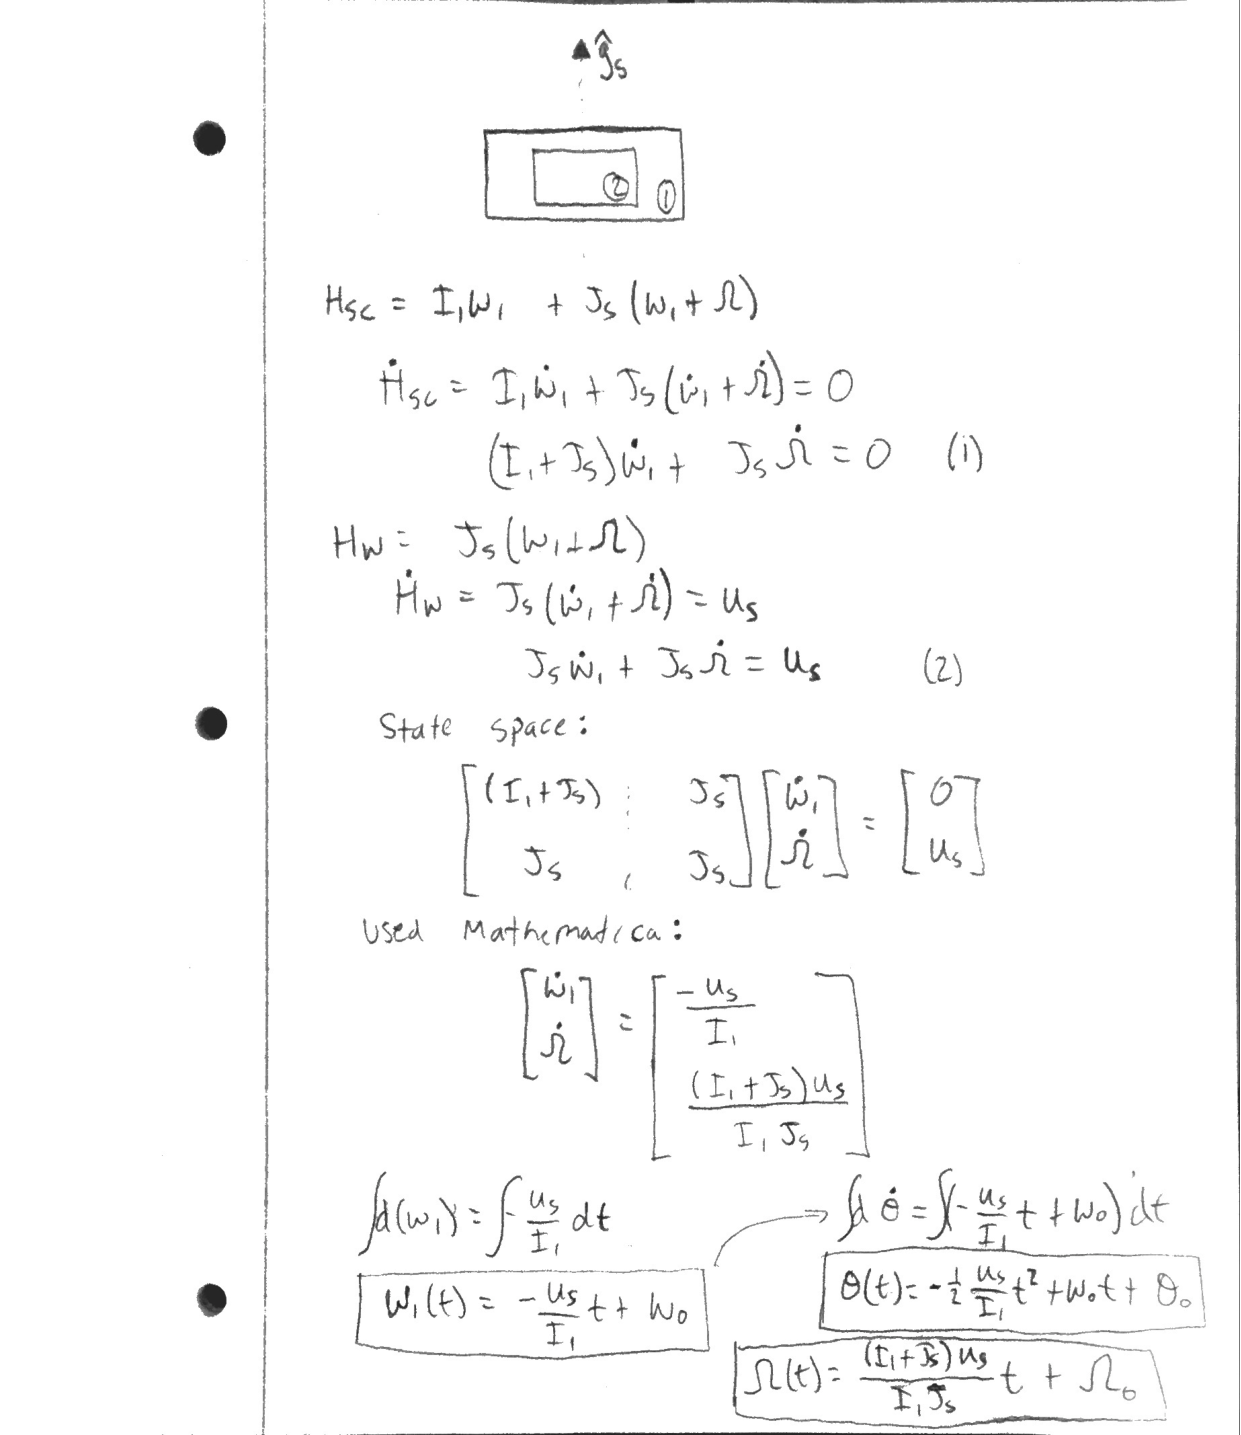
\includegraphics[width=0.8\textwidth]{Figures/BOE}}
	\caption{Back of the envelope calculation for RWs}
	\label{fig:BOE}
\end{figure}

\clearpage

\subsection{Friction Scenario - Integrated Test}

In this test the goal is to validate that the friction model is matching the desired coulomb and linear friction model. This is done by setting a spacecraft with two identical reaction wheels with identical spin axes. The spacecraft is set to have no initial rotation. The wheel speeds are equal in magnitude but opposite in direction. The expected results are that the spacecraft will not rotate and the wheel speeds will spin down to zero, and the friction forces will match the desired coulomb and linear friction model seen in Figure~\ref{fig:FrictionTorque}.

\begin{figure}[htbp]
	\centerline{
		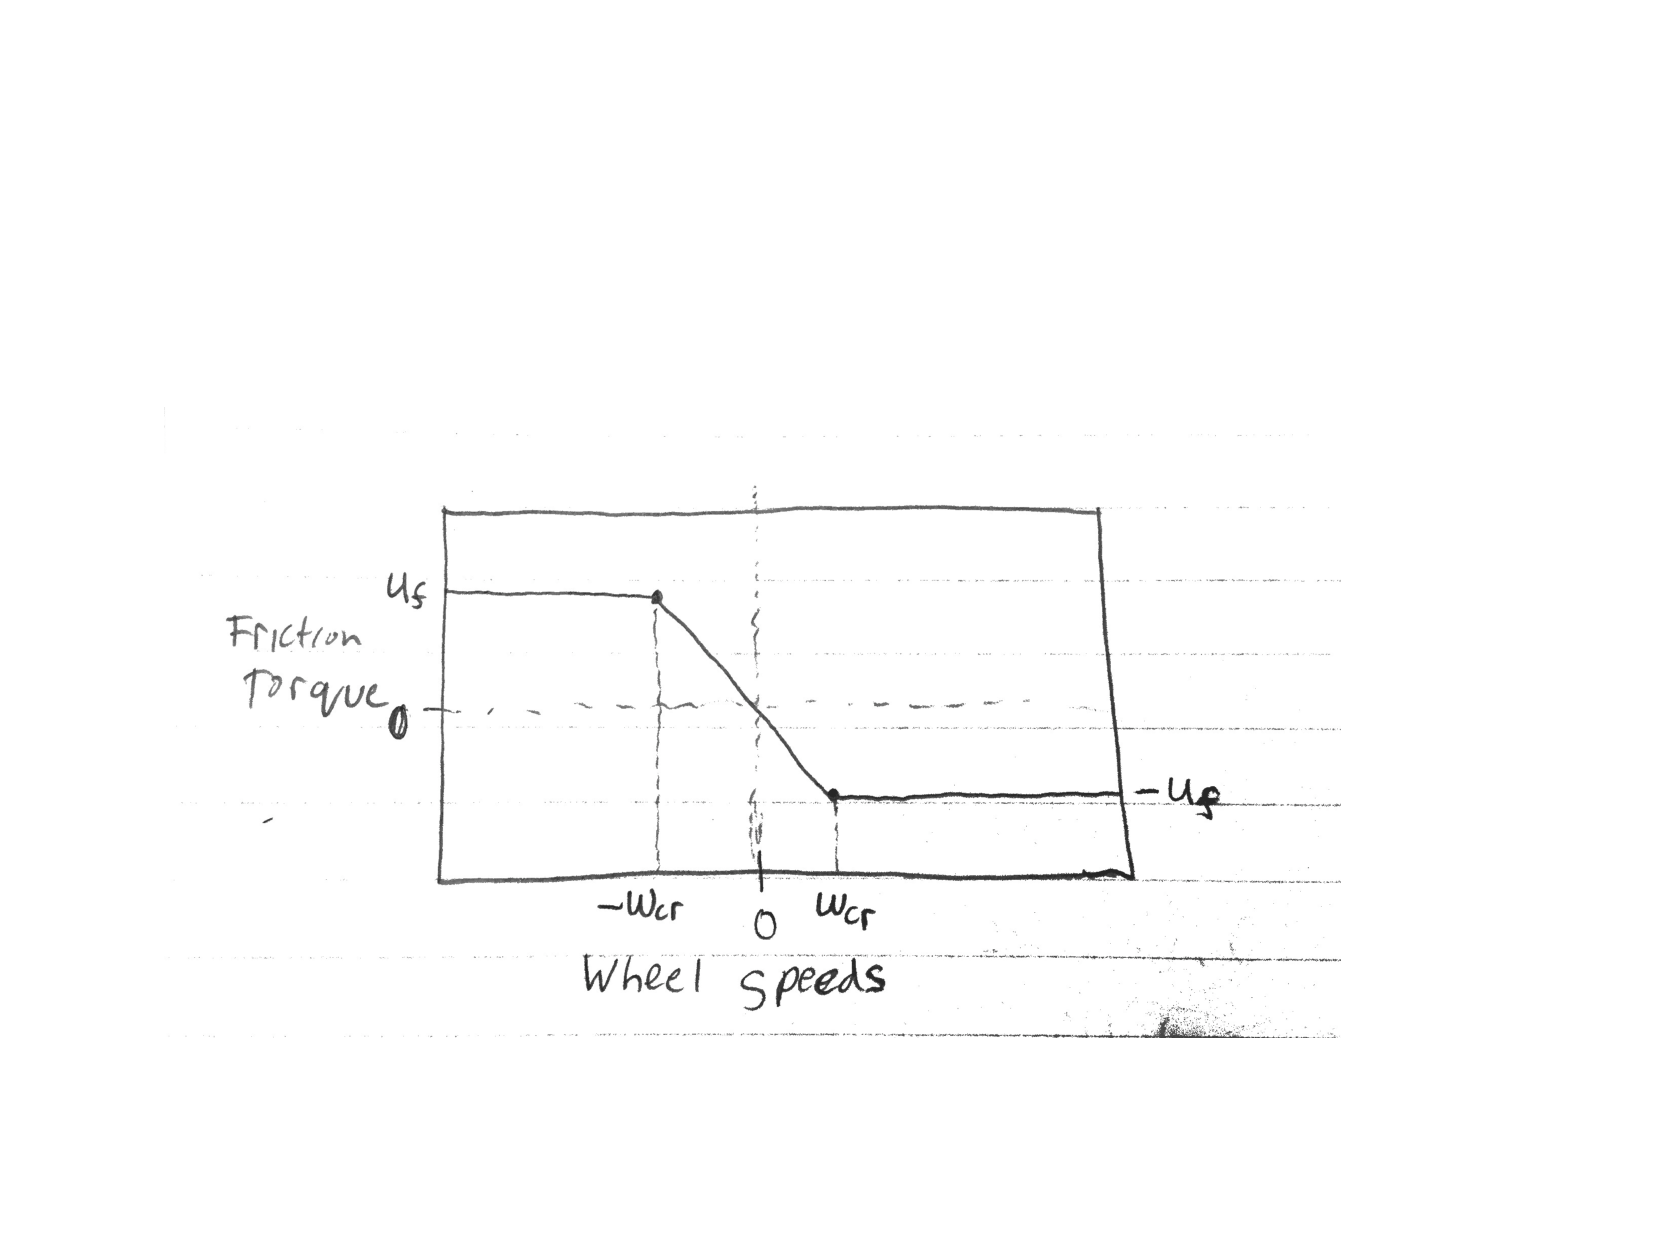
\includegraphics[width=0.8\textwidth]{Figures/FrictionTorque}}
	\caption{Friction Torque Model}
	\label{fig:FrictionTorque}
\end{figure}

\subsection{Saturation - Unit Test}

This test is ensuring that when a commanded torque requests a torque above the max torque of the wheels, the applied torque is set to the max torque. The logic can be seen in the following equation:

\begin{equation}
\begin{gathered}
\begin{aligned}
&\textnormal{\textbf{if}}\quad u_{\textnormal{cmd}} > u_{\textnormal{max}}  \quad \textnormal{\textbf{then}}\\
&\quad u_s = u_{\textnormal{max}} \\
&\textnormal{\textbf{else if}}\quad u_{\textnormal{cmd}} < - u_{\textnormal{max}}  \quad \textnormal{\textbf{then}}\\
&\quad u_s =  - u_{\textnormal{max}} \\
&\textnormal{\textbf{else}}\\
&\quad u_s = u_{\textnormal{cmd}}\\
&\textnormal{\textbf{end if}}\\
\end{aligned}
\end{gathered}
\label{eq:ballin}
\end{equation}

The test gives two commanded torques, one above $u_{\textnormal{max}}$ and one below, and ensures that the correct values are being set for $u_s$.

\subsection{Minimum Torque - Unit Test}

This test is ensuring that when a commanded torque requests a torque below the minimum torque of the wheels, the applied torque is set to zero. The logic can be seen in the following equation:

\begin{equation}
\begin{gathered}
\begin{aligned}
&\textnormal{\textbf{if}}\quad \vert u_{\textnormal{cmd}} \vert < u_{\textnormal{min}}  \quad \textnormal{\textbf{then}}\\
&\quad u_s = 0.0 \\
&\textnormal{\textbf{end if}}\\
\end{aligned}
\end{gathered}
\label{eq:ballin2}
\end{equation}

The test gives two commanded torques, one above $u_{\textnormal{min}}$ and one below, and ensures that the correct values are being set for $u_s$.

\section{Test Parameters}

Since this is an integrated test, the inputs to the test are the physical parameters of the spacecraft along with the initial conditions of the states. These parameters are outlined in Tables~\ref{tab:hub}-~\ref{tab:initial}. Additionally, the error tolerances can be seen in Table~\ref{tab:errortol}.

\begin{table}[htbp]
	\caption{Spacecraft Hub Parameters for Energy Momentum Conservation Scenarios}
	\label{tab:hub}
	\centering \fontsize{10}{10}\selectfont
	\begin{tabular}{ c | c | c | c } % Column formatting, 
		\hline
		\textbf{Name}  & \textbf{Description}  & \textbf{Value} & \textbf{Units} \\
		\hline
		mHub  & mass & 750.0 & kg \\
		IHubPntBc\_B & Inertia in $\cal{B}$ frame & $\begin{bmatrix}
		900.0 & 0.0 & 0.0\\
		0.0 & 800.0 & 0.0\\
		0.0 & 0.0 & 600.0
		\end{bmatrix}$ & kg-m$^2$ \\
		r\_BcB\_B & CoM Location in $\cal{B}$ frame & $\begin{bmatrix}
		-0.0002 & 0.0001 & 0.1 \end{bmatrix}^T$ & m \\
		\hline
	\end{tabular}
\end{table}

\begin{table}[htbp]
	\caption{Reaction Wheel 1 Parameters for Energy Momentum Conservation Scenarios}
	\label{tab:rw1}
	\centering \fontsize{10}{10}\selectfont
	\begin{tabular}{ c | c | c | c } % Column formatting, 
		\hline
		\textbf{Name}  & \textbf{Description}  & \textbf{Value} & \textbf{Units} \\
		\hline
		Js  & Spin Axis Inertia & 0.159 & kg-m$^2$ \\
		mass & mass & 12.0 & kg \\
		U\_s & Static Imbalance & 4.8E-6 & kg-m \\
		U\_d & Dynamic Imbalance & 15.4E-7 & kg-m$^2$ \\
		gsHat\_B & Spin Axis in $\cal{B}$ frame & $\begin{bmatrix}
		1.0 & 0.0 & 0.0 \end{bmatrix}^T$ & 1 \\
		rWB\_B & Location of Wheel in $\cal{B}$ frame & $\begin{bmatrix}
		0.1 & 0.0 & 0.0 \end{bmatrix}^T$ & m \\
		\hline
	\end{tabular}
\end{table}

\begin{table}[htbp]
	\caption{Reaction Wheel 2 Parameters for Energy Momentum Conservation Scenarios}
	\label{tab:rw2}
	\centering \fontsize{10}{10}\selectfont
	\begin{tabular}{ c | c | c | c } % Column formatting, 
		\hline
		\textbf{Name}  & \textbf{Description}  & \textbf{Value} & \textbf{Units} \\
		\hline
		Js  & Spin Axis Inertia & 0.159 & kg-m$^2$ \\
		mass & mass & 12.0 & kg \\
		U\_s & Static Imbalance & 4.8E-6 & kg-m \\
		U\_d & Dynamic Imbalance & 15.4E-7 & kg-m$^2$ \\
		gsHat\_B & Spin Axis in $\cal{B}$ frame & $\begin{bmatrix}
		0.0 & 1.0 & 0.0 \end{bmatrix}^T$ & 1 \\
		rWB\_B & Location of Wheel in $\cal{B}$ frame & $\begin{bmatrix}
		0.0 & 0.1 & 0.0 \end{bmatrix}^T$ & m \\
		\hline
	\end{tabular}
\end{table}

\begin{table}[htbp]
	\caption{Reaction Wheel 3 Parameters for Energy Momentum Conservation Scenarios}
	\label{tab:rw3}
	\centering \fontsize{10}{10}\selectfont
	\begin{tabular}{ c | c | c | c } % Column formatting, 
		\hline
		\textbf{Name}  & \textbf{Description}  & \textbf{Value} & \textbf{Units} \\
		\hline
		Js  & Spin Axis Inertia & 0.159 & kg-m$^2$ \\
		mass & mass & 12.0 & kg \\
		U\_s & Static Imbalance & 4.8E-6 & kg-m \\
		U\_d & Dynamic Imbalance & 15.4E-7 & kg-m$^2$ \\
		gsHat\_B & Spin Axis in $\cal{B}$ frame & $\begin{bmatrix}
		0.0 & 0.0 & 1.0 \end{bmatrix}^T$ & 1 \\
		rWB\_B & Location of Wheel in $\cal{B}$ frame & $\begin{bmatrix}
		0.0 & 0.0 & 0.1 \end{bmatrix}^T$ & m \\
		\hline
	\end{tabular}
\end{table}

\begin{table}[htbp]
	\caption{Initial Conditions for Energy Momentum Conservation Scenarios}
	\label{tab:initial}
	\centering \fontsize{10}{10}\selectfont
	\begin{tabular}{ c | c | c | c } % Column formatting, 
		\hline
		\textbf{Name}  & \textbf{Description}  & \textbf{Value} & \textbf{Units} \\
		\hline
		(RW 1) OmegaInit  & (RW 1) Initial $\Omega$ & 500 & RPM \\
		(RW 2) OmegaInit  & (RW 2) Initial $\Omega$ & 200 & RPM \\
		(RW 3) OmegaInit  & (RW 3) Initial $\Omega$ & -150 & RPM \\
		r\_CN\_NInit & Initial Position of S/C & $\begin{bmatrix}
		-4020339 &	7490567 & 5248299 
		\end{bmatrix}^T$ & m \\
		v\_CN\_NInit & Initial Velocity of S/C & $\begin{bmatrix}
		-5199.78 & -3436.68 & 1041.58
		\end{bmatrix}^T$ & m/s \\
		sigma\_BNInit & Initial MRP of $\cal{B}$ frame & $\begin{bmatrix}
		0.0 & 0.0 & 0.0
		\end{bmatrix}^T$ & - \\
		omega\_BN\_BInit & Initial Angular Velocity of $\cal{B}$ frame & $\begin{bmatrix}
		0.08 & & 0.01 & 0.0
		\end{bmatrix}^T$ & rad/s \\
		\hline
	\end{tabular}
\end{table}

\begin{table}[htbp]
	\caption{Error Tolerance - Note: Relative Tolerance is $\textnormal{abs}(\frac{\textnormal{truth} - \textnormal{value}}{\textnormal{truth}}$)}
	\label{tab:errortol}
	\centering \fontsize{10}{10}\selectfont
	\begin{tabular}{| c | c |} % Column formatting, 
		\hline
		Test   & Relative Tolerance \\
		\hline
		Energy and Momentum Conservation & 1e-10 \\
		\hline
		Position, Attitude Check & 1e-7 \\
		\hline
		BOE & 1e-8 \\
		\hline
		Friction & 1e-8 \\
		\hline
		Saturation & 1e-10 \\
		\hline
		Minimum Torque & 1e-10 \\
		\hline	
	\end{tabular}
\end{table}

\clearpage

\section{Test Results}

\subsection{Balanced Wheels Scenario - Integrated Test Results}

\input{AutoTex/ChangeInOrbitalAngularMomentumBalancedWheels}
\input{AutoTex/ChangeInOrbitalEnergyBalancedWheels}
\input{AutoTex/ChangeInRotationalAngularMomentumBalancedWheels}
\input{AutoTex/ChangeInRotationalEnergyBalancedWheels}

\clearpage

\subsection{Fully Coupled Jitter Scenario - Integrated Test Results}

\input{AutoTex/ChangeInOrbitalAngularMomentumJitterFullyCoupled}
\input{AutoTex/ChangeInOrbitalEnergyJitterFullyCoupled}
\input{AutoTex/ChangeInRotationalAngularMomentumJitterFullyCoupled}
\input{AutoTex/ChangeInRotationalEnergyJitterFullyCoupled}

\clearpage

\subsection{BOE Calculation Scenario - Integrated Test Results}

\input{AutoTex/ReactionWheelBOETheta}
\input{AutoTex/ReactionWheelBOEBodyRate}
\input{AutoTex/ReactionWheelBOERWRate}

\clearpage

\subsection{Friction Scenario - Integrated Test Results}

\input{AutoTex/ReactionWheelFrictionTestBodyRates}
\input{AutoTex/ReactionWheelFrictionTestFrictionTorque}
\input{AutoTex/ReactionWheelFrictionTestWheelSpeed}

\clearpage

\subsection{Simple Jitter, Saturation and Minimum Torque Tests Results}

\begin{table}[htbp]
	\caption{Test results.}
	\label{tab:results}
	\centering \fontsize{10}{10}\selectfont
	\begin{tabular}{c | c } % Column formatting, 
		\hline
		\textbf{Test} 				    & \textbf{Pass/Fail}  \\ \hline
		Simple Jitter  & \textcolor{ForestGreen}{PASSED}\\
		Saturation  & \textcolor{ForestGreen}{PASSED}   \\ 
		Minimum Torque  &\textcolor{ForestGreen}{PASSED}  \\ \hline
	\end{tabular}
\end{table}

\clearpage
